\section{RESULTS AND DISCUSSION}

%============================================================================
\subsection{Hardware Assembly}
\hspace{1.27cm}
The hardware assembly phase involved the integration of all mechanical, electrical, and control components to form the complete Delta robot system. This stage validated the design decisions made during the methodology phase and prepared the robot for testing.

\subsubsection{Mechanical Assembly}
\hspace{1.27cm}
The Delta robot frame was assembled using aluminum profiles for the fixed base and 3D-printed PLA parts for the arm linkages and moving platform. The three upper arms (length $r_f = 200$\,mm) are connected to the RobStride RS-00 motor shafts via custom motor mounts. The lower arm parallelograms (length $r_e = 400$\,mm) use ball joints at both ends to allow free rotation while constraining the moving platform to pure translational motion. The moving platform (side $e = 35$\,mm) carries the pneumatic solenoid gripper. The fixed base triangle (side $f = 157$\,mm) provides the reference coordinate frame for all kinematic calculations.

\par
\begin{figure}[h]
    \centering
    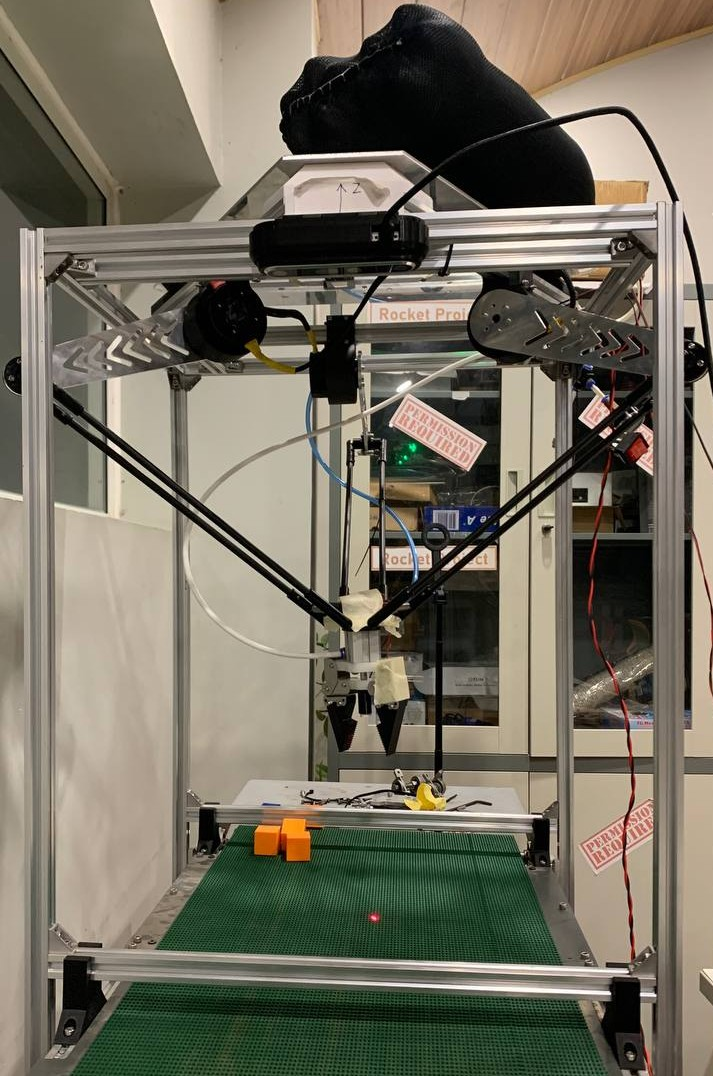
\includegraphics[width=0.45\linewidth]{image/completedAssemblied.jpg}
    \hfill
    \includegraphics[width=0.45\linewidth]{image/completedAssem.png}
    \caption{Delta Robot Complete Assembly: fabricated prototype (left)
             and CAD reference (right).}
    \label{fig:robot_assembly}
\end{figure}

\subsubsection{Electrical and Control Assembly}
\hspace{1.27cm}
Three RobStride RS-00 quasi-direct-drive motors (CAN IDs 1, 2, 3) are connected in a CAN bus daisy chain at 1\,Mbit/s. A USB-to-CAN adapter (SocketCAN, \texttt{can0}) interfaces the motors to the host computer. The pneumatic solenoid gripper is driven by motor driver CAN ID\,4 (open: \texttt{004\#00}, close: \texttt{004\#01}). The Intel RealSense D455 camera is connected via USB\,3.0 and powered independently. A 24\,V power supply feeds the motor drivers; the host computer runs Ubuntu 22.04 with ROS\,2 Humble.

\par
\begin{figure}[h]
    \centering
    % \includegraphics[width=0.7\linewidth]{image/electronics_assembly.jpg}
    \caption{Electronics and CAN Bus Assembly.}
    \label{fig:electronics_assembly}
\end{figure}

%============================================================================
\subsection{Kinematic Validation}
\hspace{1.27cm}
The kinematic model was validated by commanding the robot to a set of known positions and comparing the FK-computed end-effector position against the commanded position.

\subsubsection{Forward Kinematics Validation}
\hspace{1.27cm}
For each commanded position $(x, y, z)$, the IK solver computed joint angles $(\theta_1, \theta_2, \theta_3)$, which were sent to the motors. Motor encoder feedback was read back, FK was applied to the measured angles, and the position error was computed. Results from a representative set of test positions are shown in \textbf{\autoref{tab:fk_validation}}.

\begin{table}[ht]
    \centering
    \caption{Forward Kinematics Validation Results.}
    \label{tab:fk_validation}
    \small{
    \begin{tabular}{ccccccccc}
        \textbf{Test} & $\theta_1$($^\circ$) & $\theta_2$($^\circ$) & $\theta_3$($^\circ$) & $x$ (mm) & $y$ (mm) & $z$ (mm) & \textbf{FK err} (mm) \\
        \hline
        1 & 7.3  & 7.3  & 7.3  &   0.0 &    0.0 & $-$350.0 & 0.39 \\
        2 & 22.4 & 22.4 & 22.4 &   0.0 &    0.0 & $-$410.0 & 0.36 \\
        3 & 26.2 & 12.1 & 36.3 &  88.0 &    6.0 & $-$410.0 & 0.44 \\
        4 & 34.2 & 15.0 &  8.2 & $-$22.5 & 91.4 & $-$385.0 & 0.47 \\
        5 & 5.4  & 42.1 & 42.1 &   0.0 & $-$150.0 & $-$410.0 & 0.45 \\
        6 & 30.1 &  9.0 & 43.9 & 127.5 &  10.5 & $-$410.0 & 0.39 \\
        \ChangeRT{1.5pt}
    \end{tabular}}
\end{table}

\hspace{1.27cm}
FK position errors were consistently below 0.5\,mm across all tested configurations, confirming that the kinematic model is accurate and the motor encoder feedback is reliable. The maximum observed error of 0.47\,mm is well within the tolerance required for pick-and-place operations with the pneumatic gripper.

\subsubsection{Inverse Kinematics Validation}
\hspace{1.27cm}
IK solutions were pre-checked before every pick sequence. All approach, pick, lift, and home positions were verified reachable (IK status = 0) before commanding any motion. The joint angle constraint $\theta_i \geq 0$ was enforced to prevent physically unreachable configurations. No IK failures were observed during normal operation within the $\pm150$\,mm planar workspace at pick depth $Z = -410$\,mm.

%============================================================================
\subsection{Vision Pipeline Results}

\subsubsection{Camera Calibration}
\hspace{1.27cm}
Camera-to-robot transform calibration was performed iteratively using a projected workspace overlay rendered in the camera feed. The overlay projects the four workspace corners (at $(\pm150, \pm150, -490)$\,mm platform frame) through the inverse transform to image pixels, drawing the green workspace box and a white crosshair at the projected $(0, 0)$ origin. By adjusting \texttt{CAM\_TX\_MM = -10.0}\,mm and \texttt{CAM\_TY\_MM = +235.0}\,mm until the crosshair aligned with the laser dot at the robot home position, the transform was calibrated. The calibrated translation vector is:
\begin{equation*}
    \mathbf{t} = [-10.0,\; +235.0,\; -20.0]^\top \text{ mm}.
\end{equation*}

\subsubsection{Object Detection}
\hspace{1.27cm}
The HSV orange\_blob detector achieved consistent detection 
with a reported confidence of 1.00 across all tested 
lighting conditions, with a processing time of 3--16\,ms 
per frame at 13--31\,fps on CPU. The deterministic nature 
of HSV filtering provided zero false positives for the 
orange test object against the green cutting mat background.


%============================================================================
\subsection{Pick-and-Place Task}
\hspace{1.27cm}
A complete pick-and-place operation was performed to evaluate the performance of the developed Delta robot. The task involved detecting a stationary orange object, applying the visual EE feedforward correction loop, descending to pick depth ($Z_{\text{pick}} = -535$\,mm platform), grasping, transporting to the drop position at $(150,\, -150,\, -500)$\,mm platform (belt exit), and returning to home.

\par
\hspace{1.27cm}
The 8-state FSM executed the full sequence:
IDLE $\to$ APPROACHING $\to$ PICKING $\to$ GRASPING $\to$ LIFTING $\to$ TRANSPORTING $\to$ DROPPING $\to$ RESETTING $\to$ IDLE,
consistent with the FSM described in \autoref{sec:task_framework}.
\begin{figure}[h]
    \centering
    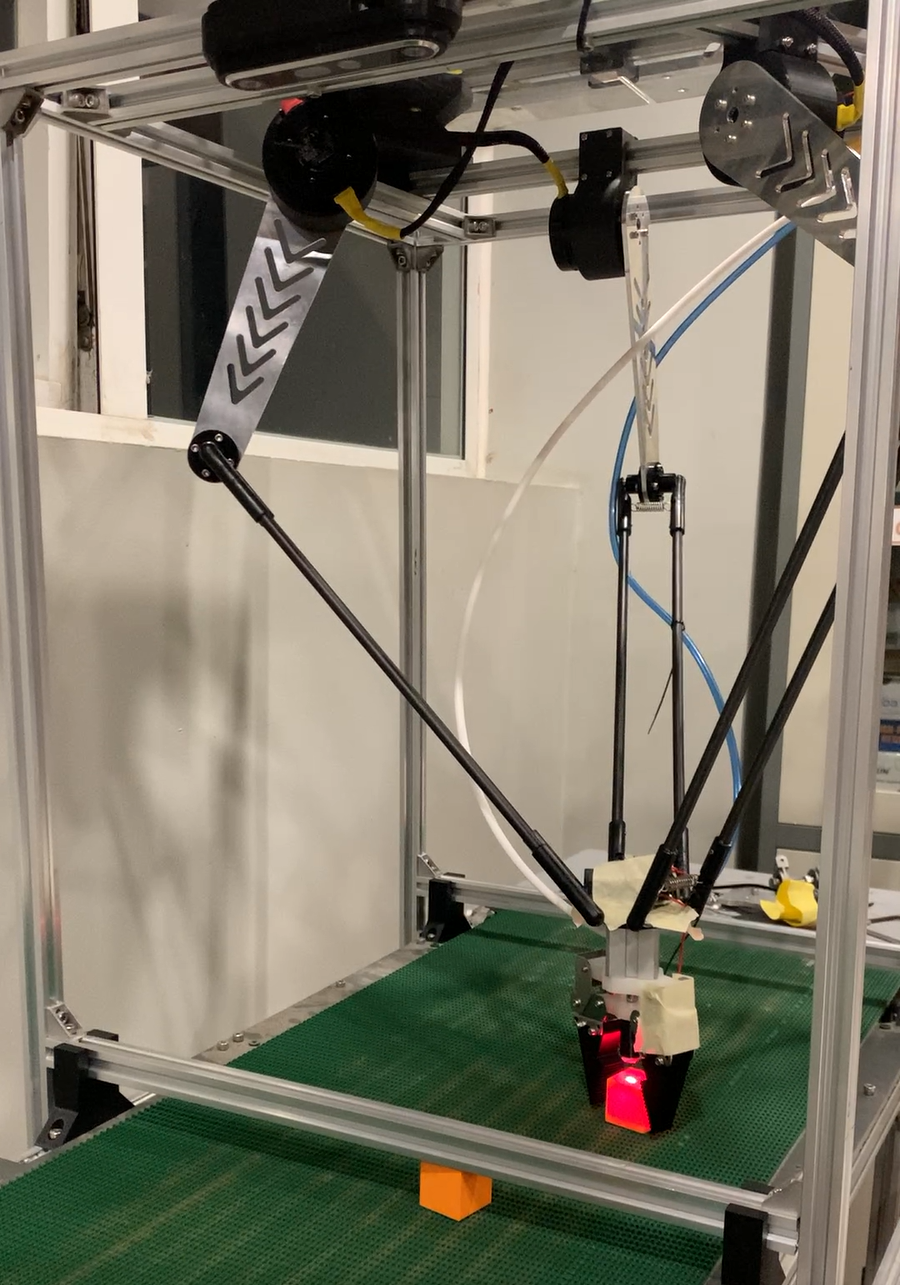
\includegraphics[height=6.5cm]{image/picking.png}
    \hspace{5mm}
    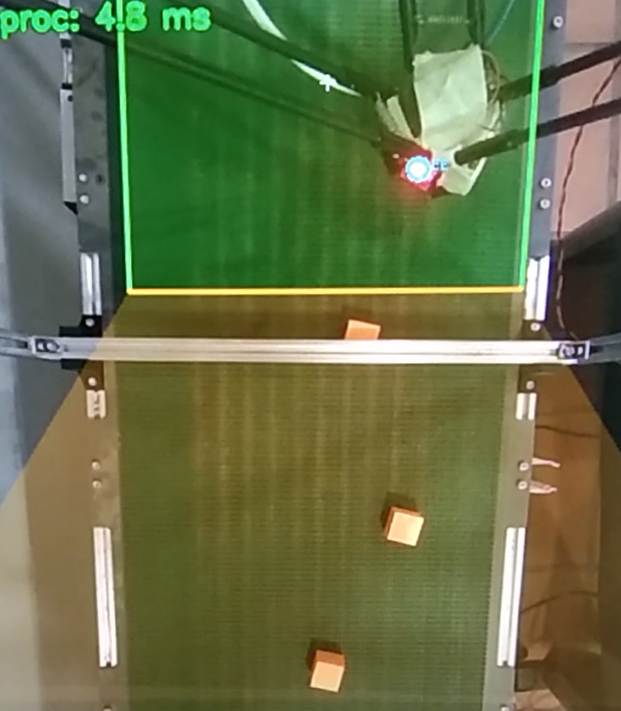
\includegraphics[height=6.5cm]{image/vspicking.png}
    \caption{Robot EE Approaching Object with Visual Correction Active:
             Physical Picking (left) and Visualization EE Correction
             Picking (right).}
    \label{fig:pick_task}
\end{figure}

\begin{figure}[h]
    \centering
    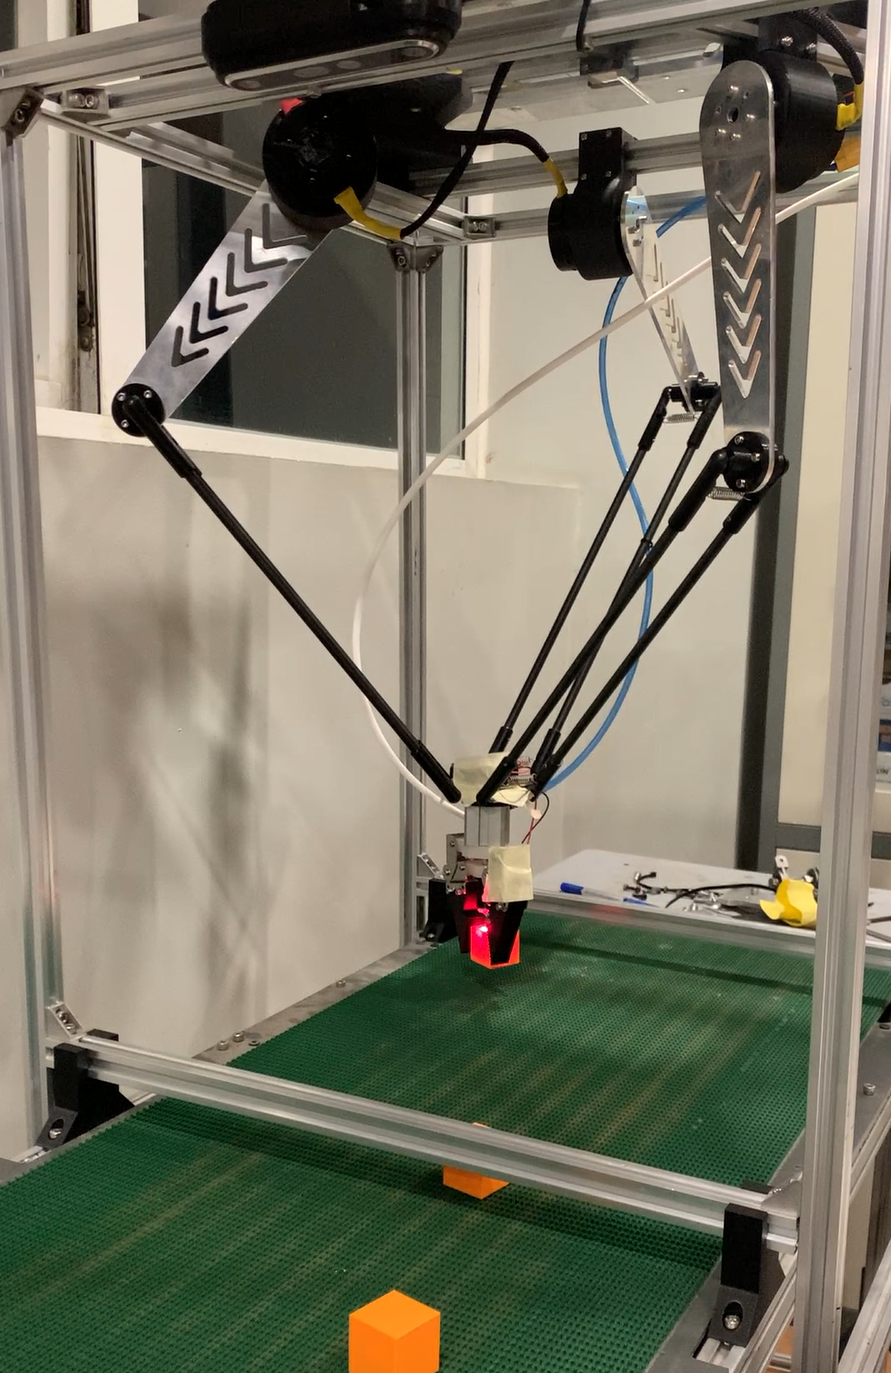
\includegraphics[height=6.5cm]{image/placing.png}
    \hspace{5mm}
    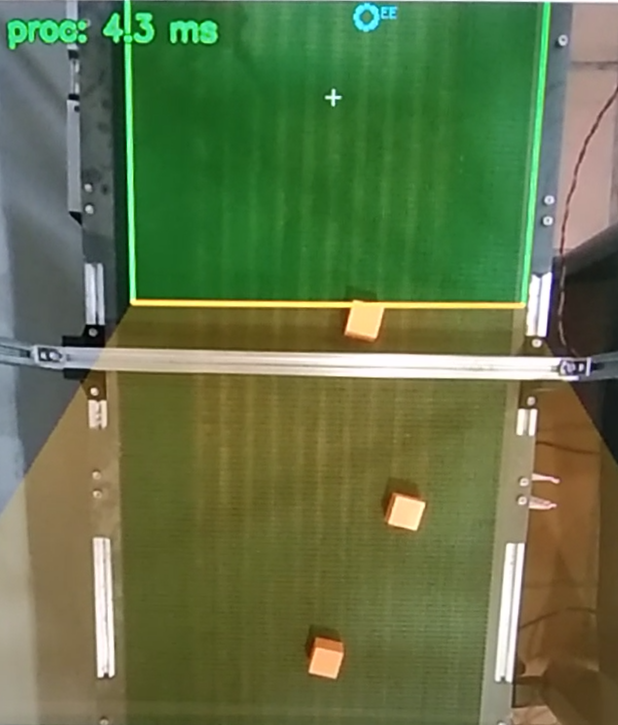
\includegraphics[height=6.5cm]{image/vsplacing.png}
    \caption{Robot Placing Object at Belt Exit Position: Physical
             Placing (left) and Visualization EE Correction
             Placing (right).}
    \label{fig:place_task}
\end{figure}

\subsubsection{Visual EE Correction Results}
\hspace{1.27cm}
The feedforward correction loop successfully reduced the X-axis error from an initial value of approximately 17--40\,mm to below the 3\,mm convergence threshold (\texttt{EE\_CORRECTION\_THRESH\_MM = 3.0}) within 2--4 iterations. A representative correction sequence is shown below:

\begin{table}[ht]
    \centering
    \caption{Representative EE Correction Iteration Results.}
    \label{tab:ee_correction_results}
    {\small
    \begin{tabular}{ccccc}
        \textbf{Iter} & $\Delta x$ (mm) & $\Delta y$ (mm) & \textbf{dist} (mm) & \textbf{Action} \\
        \hline
        0 & +17.7 & +37.5 & 41.5 & Move X corrected \\
        1 & +7.9  & +39.5 & 40.2 & Move X corrected \\
        2 & +3.9  & +37.5 & 37.7 & X converged      \\
        — & —     & —     & —    & Descend to pick  \\
        \ChangeRT{1.5pt}
    \end{tabular}}
\end{table}

\hspace{1.27cm}
Y-axis correction was implemented but showed oscillation on the moving belt due to object displacement during iteration. For stationary objects, XY correction converged reliably. Further tuning of the Y-axis correction strategy is identified as future work.

%============================================================================
\subsection{Performance Summary}
\hspace{1.27cm}
The overall performance of the Delta robot system is summarised in \textbf{\autoref{tab:performance_summary}}.

\begin{table}[ht]
    \centering
    \caption{Performance Summary.}
    \label{tab:performance_summary}
    \small{
    \begin{tabular}{lcc}
        \textbf{Parameter} & \textbf{Design Target} & \textbf{Achieved} \\
        \hline
        FK positional error       & $<$1.0\,mm      & $<$0.5\,mm        \\
        Motion preset             & medium          & medium            \\
        EEF $v_{\max}$            & 2000\,mm/s      & 2000\,mm/s        \\
        EEF $a_{\max}$            & 5000\,mm/s$^2$  & 5000\,mm/s$^2$   \\
        Workspace (planar)        & $\pm$150\,mm    & $\pm$150\,mm      \\
        Workspace (vertical)      & 177\,mm         & $-$323 to $-$500\,mm \\
        Belt speed (measured)     & —               & 12.85\,mm/s       \\
        Belt prediction offset    & —               & $\leq$8.3\,mm     \\
        EE correction convergence & $<$5\,mm        & $<$5\,mm (X-axis) \\
        Detection confidence      & $>$0.9          & 1.00              \\
        Detection FPS             & 15\,fps         & 13--31\,fps       \\
        CAN bus baudrate          & 1\,Mbit/s       & 1\,Mbit/s         \\
        \ChangeRT{1.5pt}
    \end{tabular}}
\end{table}

\hspace{1.27cm}
The FK error below 0.5\,mm confirms excellent mechanical accuracy and encoder reliability of the RobStride RS-00 actuators. The visual EE correction loop effectively compensates for non-linear transform residuals across the workspace. The primary open item is completion of the non-linear error map calibration (\texttt{measure\_error\_grid.py}) which would further reduce systematic errors across all workspace positions.
